\subsection{Effective Shear Wave Velocity Range}

There is not a unique solution for \qsvs{} input parameters. Many combinations of the parameters can provide similar $Q$ and, consequently, accurate results. Although we define the anelasiticy as a function of the shear wave velocity, ground motion simulation model generates a Q value based on provided input parameters. As an example if we consider a domain with \vs{}=1500~m/s, and $Q=$~120 which is measured for the region, all the \qsvs{} relationships that are shown in Table~\ref{tab:example_effective_vs} are considered acceptable. 

\begin{table}[ht]
\centering
\caption{Example of acceptable parameters for  a domain with $Q$~=120 and \vs{}=1500~m/s}
\label{tab:example_effective_vs}
\begin{tabular}{ccc}
C  & $\alpha$ & $\beta$ \\ \hline
5   & 20                    & 4.3141               \\
10 & 25                    & 3.6541               \\
15 & 30                    & 3.0897               \\
20 & 35                    & 2.5892               \\
25 & 40                    & 2.1333              
\end{tabular}
\end{table}

Fig.~\ref{fig:example_acceptable_parameters} illustrates Table~\ref{tab:example_effective_vs} parameters. For ground motion simulation models only $Q$ value (which is 120 in this example) is important. Obviously, infinite combination of parameters can generate the objective $Q$ value. 

 \begin{figure}[ht]
    \centering
    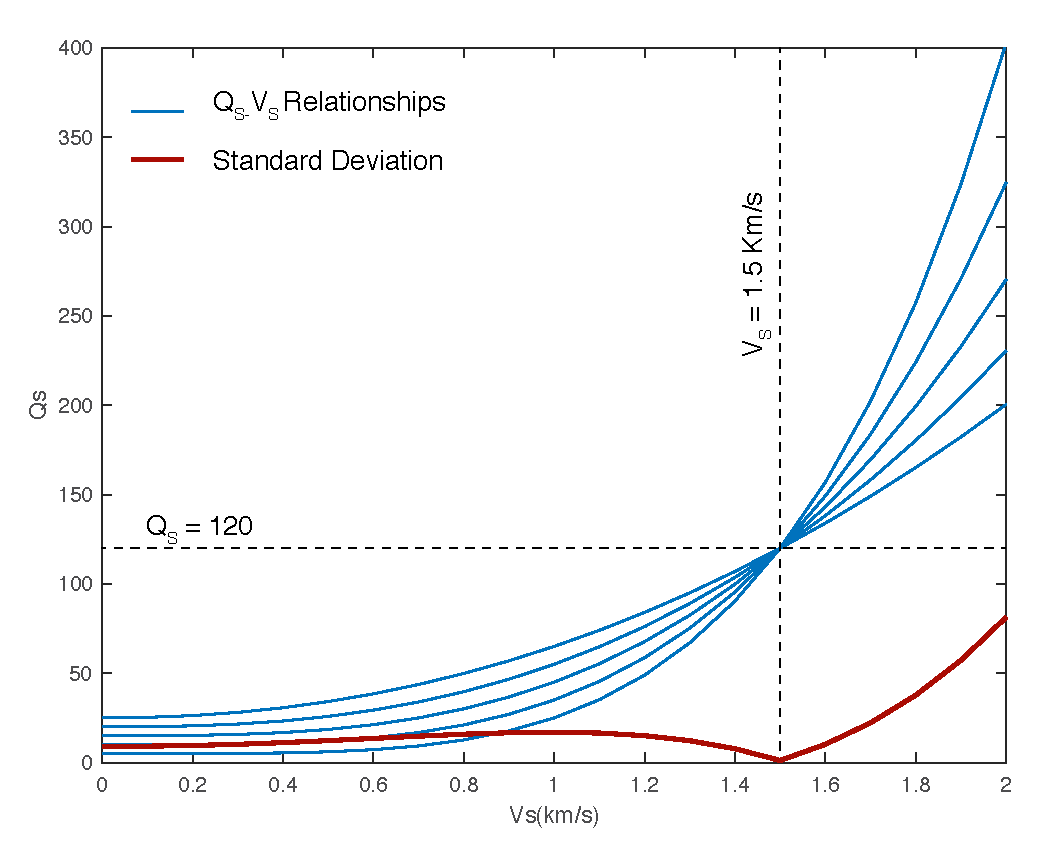
\includegraphics[width=0.5\textwidth]{figures/pdf/Figure_04.pdf}
    \caption{Example of acceptable solutions for constant \qs{} value. Blue thin lines are plotted based on Table~\ref{tab:example_effective_vs} parameters. Red thick line is standard deviation of \qs{} values. Standard deviation is the minimum value at the convergence point.}
    \label{fig:example_acceptable_parameters}
\end{figure}

Therefore, the optimization process, with respect to the shear wave velocity range of each station will find a set of appropriate parameters. With repeating the optimization process and plotting the results, we indicate the effective shear wave velocity range by computing standard deviation of the $Q$ values for each \vs{}. Standard deviation, in this context, is a proxy to measure the level of convergence. We consider two main conditions to accept the results of optimization processes:

\begin{itemize}
\item If synthetic solutions converge at a range of shear wave velocities
\item If the optimization process successfully locate the input parameters
\end{itemize}
 
 Application of standard deviation can address the first condition. The second condition is the research question of this study. We do not know the $Q$ values for the study region. However, we can follow several steps to estimate the capability of the optimization process.  The mean value of all converged solution can be considered as a potential answer to the research question because it has the same values at the convergence point as other solutions. Therefore, We use that $Q$ values and run ground motion simulations and assign the results as a target value. This time we run the optimization process with the new target value. If the converged points are the same as initial parameters (i.e., $Q$ values according to used $C$, $\alpha$, $\beta$ for target simulation), we accept the first results that come from optimization process for actual observation. If the convergence points and used $Q$ values do not coincide we reject the solutions. In other words, we study whether the optimization process is capable of finding appropriate parameters while the target $Q$ is close to mean $Q$ values. Some stations provide a convergence point different than actual parameters. One reason can be the metrics that we use. Maybe they are not adequate for some stations signals. More research is ongoing in this section. Whatever the reason is, if we do not trust the process for a specific station, we ignore the results of the process. 
 

